\chapter{Impedance estimation}
\label{chap:estimation}

The previous chapter shows how I deisgnied, applied and recorded multi-frequency electrochemical signals of drifting systems.
In this chapter I will elucidate the methods I used for the estimation of instantanous impedance from the multi-frequency signals.
Of the three methods described in the introduction, namely ST-FFT \pageref{sec:fft-eis}, DMFA \pageref{sec:dmfa} and fitting the BLTVA \pageref{sec:BLTVA}, I used in this work only the first two because of the ease of implementation with basic signal processing concepts and well enstablished use in the literature.
The novelty of this work is the introduction of a mixed method in which ST-FFT and DMFA are combined to achieved broad band frequency response function estimation while maitning the best characteristics of both and reudcing the disk space otherwise needed.
This is achieved by estimating the high-frequency band of the impedance on-line during the experiment with the ST-FFT and the remaining lower frequency band offline with DMFA.
This was possible thanks to the automation described in the previous chapter.
With the full control on the data stream and the multi-threded excecution, it is possible to perform calculations on the data recieved from the piscope.

This chapter describes how impedance is estmiated off-line with the DMFA and the downsaides of the method. 
Then I will described the signal workflow to estimate part of the impedance on-line.
The mixed method was used for the long-term broad-band characterization of li-ion commerical batteries discussed in Chapter \ref{chap:coins}, while the rest of the applications used only the off-line DMFA method (Chapters \ref{chap:LTP}, \ref{chap:capacitor}, \ref{chap:anodes}) because they where perfomred alongside the develoment of the setup.

\section{Off-line estimation with DMFA}
%Under which conditions the system can be approximated as locally LTI
%Over what window the drift is negligible
%Why the multisine period must be shorter than the drift timescale
In this work I use the term \emph{off-line} to emphasize the difference with the \emph{on-line} approach that is the subject of development.
The off-line method is the traditional method used in system identification for which input and output mutlti-frequency signals are sampled for an integer number of periods and the time-varying frequency transfer funciton is estimated though a Fourier Analysis. 
In this work I used the Dynamic Multi-Frequency Analysis (DMFA) to estimate the estimate the impedance choising a symmetric Fermi-Dirac function as fitler.
The approach is the same presented in previous work of the ESECS group [cite works].

The frequency content and the period of one multi-sine is dictated from the excitation waveform and they define the parameters of the filter of the DMFA: bandwidth and order.
As analyzed in \cite{chukwuStatisticalAnalysisMeasurement2022}, to estimate every instantaneous impedance indipendently from the privous and succesfull instants, the bandwidth must be an integer times the inverse of the multi-sine period and the order of the filter should be a number around 8. 
The latter shapes the amplitude of the side-bands of the filter.

\section{On-line processing and data reduction}
\label{On-line computation}

\subsection{Limitation of the DMFA}
Using the method of DMFA (but also fitting a BLTVA) requires storing the complete signals from beginning to end of the experiment.
When the sample rate of the acquisition is high or the experiment is long, the ammount of disk-space occupied by the signals become significant.
The sample rate is determined by the maximum frequencies of the excitation wave (at least twice according to the Nyquist Theorem) while the experiment time depend on the desired characterization of the system; charaterization of redox couple via cyclic voltammetry might last a few minutes while characterizing the intercalation in layered material takes hours, and the phenomena of battery aging appears in weeks.

The frequency dictates the ammount of data per hour to be stored.
% An fast system that express its dynamic up to a frequncy of 1kHz (for example a big battery) if voltage and current are sampled at 5kHz with a resolution of 16\,bit the disk space taken is of 72 \,MB per hour, that correspond to 1.7\,GB per day enche cycling jut one battery would fill up modest hard drives in a few weeks.

Typically, batteries and other electrochemical systems responds to escitations up to few hundred Hertz.
Sampling, for axample, the signals of as system at 500kHz creates 7.2\,GB per hour, filling up even the most spacious hard drives in a few days.
Using Dynamic Impednace with high frequency excitations and for long time become unpractical under these circumstances, especially when interested in performing replicas or parallel cells measurments with the same computer.
Furthermore, integrating the methods of Dynamic Impedance in more modest hardware like micro-computers and micro-controllers for the real time estimation of energy storage or generation devices is practically impossible.

This work provides a solution to the problem of data volume computing the impedance via Short-time Fast Fourier Transform on-line on the high frequency band. 
The short-time FFT has a frequency resolution that is the invers of the windows length, while the DMFA has the frequency resolution of the inverse of the entire signal lenght. 
This means that the first is not adeguate to estimate the low frequency band and furthrmore it is not capable of separating the excitation frequency response from the drift.
The solution is to use the FFT of a short window and estimate the impedance for the frequencies that are fast enough to consider the system "frozen" in time. 
For example, in chapter \ref{chap:coins} I show Li-ion batteries cycle at C/10 with the FFT applied on a window of 100s where only the impedance for the frequencies componets above 10Hz is estimated.
Such components oscillates a full period 1,000 to 100,000,000 times during the 100s window hence their frequency analysis shows sharp and defined peaks beacase everaging over so many periods and the system can be considered statinoary.
Saving this information for hours is redundant, therfore I developed a strategy to calculate part of the impedance on-line, low-pass filtering the signals and decimate them for a later off-line analysis with DMFA.

\subsection{Temporary stationarity of the system}
% Here goes the explanation and the figure I had in mind
This method is valid because of the assumption that there is a superimposition only of the lowest frequencies with the drift wile the high frequencies are not influenced.
In other words, for the high frequency band the system is considered stationary. 
The critical frequency that separates the frequency bands depends on the drift rate and the kinetics of the system.
One can look at the Fourier Spectrum of a signal to deduce the treshold for which the system doesn't respond anymore.

\subsection{Strategy of the on-line processing}

The on-line processing is possible thanks to a software component excecuted inside the automation software described in previous chapter which excecutes the estimation and decimation when the signal reaches the size of the desired window (ex. 100s to keep the same example as before).

When a voltage and current blocks of data equivalent to the window length are acquired, the software part in charge of the streaming copies the signals to another object that performs the processing. 
I called this new object "BlockCalculator" and added as submodule of DEIStools.
The processing performs the following actions:
\begin{itemize}
    \item remove linear baseline of both signlas;
    \item perform the DFT of the signals;
    \item estimate the impedance of the high frequency band as ratio of the two fourier spectra at the frequencies of the excitation and store it;
    \item apply a Fermi-Diract function as low-pass filter;
    \item perform inverse DFT of the filtered signals;
    \item decimate the signals and store them.
\end{itemize}
The user must choose the low-pass filter critical frequency to remove all the frequency components already estimated in the previous step. Continuing the example of before it would be all the frequencies above 10Hz, so I choose a critical frequency of 8Hz.

Later the DMFA is used to estimate impedance from 10mHz to 10Hz (exclueded) and the two are merged together to obtain the complete broadband impedance.
If the time resolution of the DMFA and the window length are the same there is no need to process the istantaneous impedances to match the time steps.

The strategy is summarized in Figure \ref{fig:online processing scheme}.
\begin{figure}[H]
    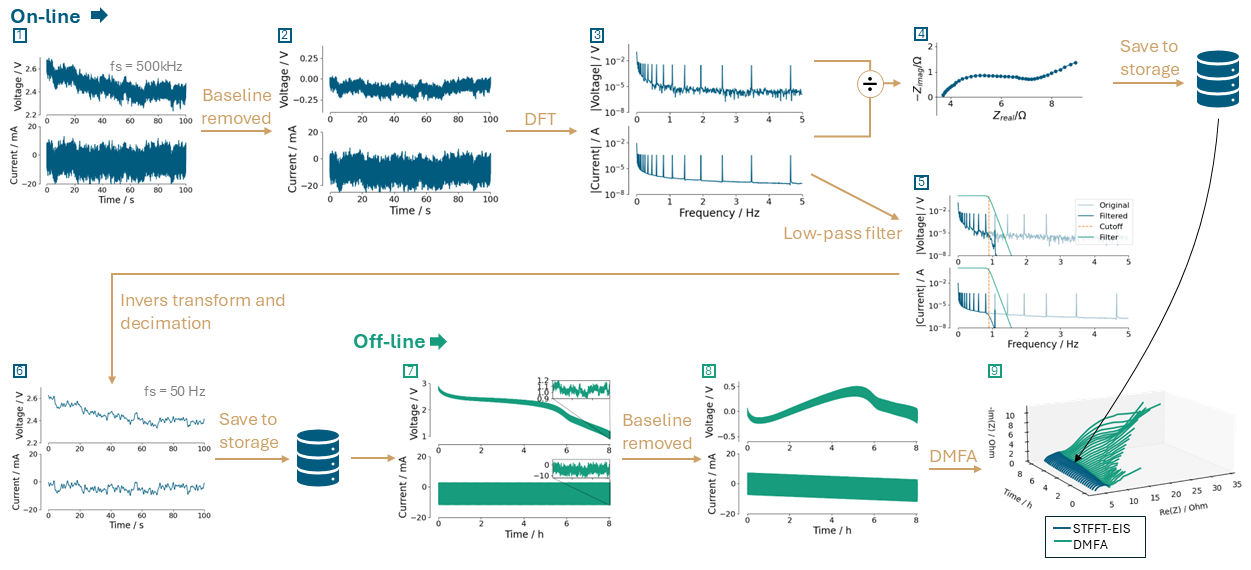
\includegraphics[width = \textwidth]{figures/estimation/computation_scheme.png}
    \caption{Schematics of the on-line processing.}
    \label{fig:online processing scheme}
\end{figure}

\section{Data exploration}
A Dynamic Impedance experiment might return dozens to thousend of istantanous spectra depending on the temporal resolution and acquisitino length. 
This is why the analysis, subject of the next chapter, is even more relevant.

\section{Limitations of this approach}
The use of a mixed method allows for a real braod-band Dynamic Impedance Spectroscopy but it brings some complications with it.
First of all the number of calculation is not a problem for a desktop computer but the method is not ready for being implemented as it is on micro-controller or micro-computer where I believe will make a tangible impact on device characterization and controll.
The ammount of calculations and memory must be optimized.
Furthermore the analyis in blocks of data creates small discontinouties of circa 6mV between two consecutives. 
This arises from the Gibb's effect.
The effect on the final impendace presents as an oscillation feature at the noise level so it doesn't disrupt the capability of DMFA to estimate the impedance. 
I don't know if the effect remains small at higher current densities.
Though it is possible to substitute the impedance calculation and low-pass filtering with a properly designed Finite Response Filter (FRF) that would be compatible with micro-controllers architecture.





% \section{Drift removal}

% In both methods, one can strongly reduce the zero-frequency skirt in the Fourier space and the Gibbs effect by removing the baseline for current and voltage signals. 
% I chose to use just a simple baseline removing because other classical methods did not work for me. 
% Typically one can use sliding window averaging, spline or polynomial fitting or gaussian process regression to name the main one. 
% In my experience non of these methods could effectively decouple the trend and the first few frequencies of the multisine that are overlapping. 
% A complete Python library can be used to test these and more trend removal techniques, it is called Wotan. Hellemans and al. developed a method for de-trending signals with low frequency containing multi-sine but there is no available Python implementation to try out and the functional analysis used in the official is above my mathematical skills to implementing it myself.